\setchapterstyle{kao}
\setchapterpreamble[u]{\margintoc}

\todo{increase main text width (read in kao docu)}


\chapter{Standard Model Background Simulation and Data Processing}
\labch{simulation_and_processing}

The analysis presented in this thesis is highly dependent on an efficient event selection to reduce the raw IceCube trigger data to a usable atmospheric neutrino sample and on a precise estimation of both expected SM background and BSM signal events through MC simulations. This chapter describes the current simulation and event selection chain used for state-of-the-art IceCube neutrino oscillation measurements like \sidecite[0.3cm]{OVS_PRD}. The whole chain can be broadly split into 4 steps:

\begin{enumerate}[wide]
    
    \item[]{\textbf{Step 1} Event Generation:} The initial step for all particle (non-noise) simulation is the generation of events using chosen initial distributions and fluxes. Events are usually the primary particle and the particles produced in the interaction with the ice.

    \item[]{\textbf{Step 2} Detector Simulation:} The particles from the first step are propagated through the ice, producing Cherenkov photons, which are then propagated further. If they hit a DOM the full detector response (PMT, readout, trigger and online processing) is simulated.
    
    \item[]{\textbf{Step 3} Processing:} 
    
    \todo{add short description of the processing levels (up to L5?)}


    \item[]{\textbf{Step 4} Reconstruction:}
    
    \todo{add short description of the reconstruction (L6 to final?)}

\end{enumerate}

This chapter only describes the event generation for the SM background simulation (neutrinos and muons), while the signal simulation is described in \refch{signal_simulation}. The detector simulation is identical for both signal and background events while processing and reconstruction are applied to all simulation and data in the same way. Splitting the simulation steps has the advantage of reusing the outputs of for example the generation step to propagate the particles with different ice model, in order to estimate the systematic impacts of uncertainties of the ice properties. Similar approach can be taken for varying detector response and through this a more efficient (reduced) use of computing resources can be achieved. The following sections describe the different steps in more detail and the last section, \refsec{systematic_uncertainties}, describes the related systematic uncertainties considered for this work.


\section{Event Generation}

\todo{write bullet points into full sentences for event generation section (read another thesis for more info)}

The MC is used in the analysis by applying a method called \textit{forward folding}, where a very large number of events (signal and background) is produced using sampling distribution that are tuned to have a large selection efficiency. Those distributions don't have to be physically correct distributions, but they need to cover the full parameter space of interest for the analysis. To produce the correct physical distributions each event gets a weight, which can be used to estimate the expected number of events given a specific choice of physics and nuisance parameters. The large number of raw MC events ensures a good estimation of the expected numbers and weighted distributions. 

The analysis itself is then performed by comparing the weighted MC distributions to the observed data. This is done by binning them as will be described in \refch{analysis} and calculating a loss function comparing the bin expectations to the data. By varying the physics and nuisance parameters, that govern the weights, the loss function can be minimized and the parameters producing MC that describes the data best are found. In order to achieve a reliable result with this method the MC needs to be precise and as close to the data as possible (at least at the final selection step). 


\subsection{Neutrinos}

Due to the very low interaction rate of neutrinos, the event generation is performed in a way that forces every event to interact in a chosen sampling volume. The weight of each event is then calculated as the inverse of the simulated neutrino fluence
\begin{equation}
    w = \frac{1}{F_{\mathrm{sim}}} \frac{1}{N_{\mathrm{sim}}}
    \;,
    \labeq{neutrino_generation_weight}
\end{equation}
where $F_{\rm{sim}}$ is the number of neutrino events per energy, time, area, and solid angle and $N_{\rm{sim}}$ is the number of simulated events. If this weight is multiplied by the livetime and the theoretically expected neutrino flux for a given physical model, it results in the number of events that this event would produce. The used baseline neutrino flux computed for the South Pole is taken from \sidecite{PhysRevD.92.023004_Honda_Flux}.

The chosen simulation volume is a cylinder centered in DeepCore with radius and height chosen such that all events possibly producing a signal are contained. The different sizes are chosen depending on energy and neutrino flavor are shown in \reftab{genie_sampling_cyilinder}.
\begin{table}[h]
    \begin{center}
        \small
        \begin{tabular}{ p{1.0cm} p{1.8cm} p{1.3cm} p{1.3cm} p{1.4cm} p{0.6cm} }

            \hline\hline

            \textbf{Flavor} & \textbf{Energy [\si{\giga\electronvolt}]} & \textbf{Radius [\si{\metre}]} & \textbf{Length [\si{\metre}]} & \textbf{Events/File}  & \textbf{Files}\\ 

            \hline\hline

            \multirow{4}{*}[-1.em]{ $\nu_e+\bar{\nu_e}$ }
            & 1-4
            & \multirow{1}{*}[-1.em]{ 250 }
            & \multirow{1}{*}[-1.em]{ 500 }
            & 450000
            & \multirow{4}{*}[-1.em] {650} \\

            \cmidrule{2-2}
            \cmidrule{5-5}
            
            & 4-12
            & 
            & 
            & \multirow{1}{*}[-1.em] { 100000 }
            & \\

            \cmidrule{2-4}

            & 12-100
            & 350
            & 600
            & 
            & \\

            \cmidrule{2-5}

            & 100-10000
            & 550
            & 1000
            & 57500
            & \\

            \hline
            \hline

            \multirow{4}{*}[-1.em]{ $\nu_\mu+\bar{\nu_\mu}$ }
            & 1-5
            & 250
            & 500
            & 408000
            & \multirow{4}{*}[-1.em] {1550} \\

            \cmidrule{2-5}
            
            & 5-80
            & 400
            & 900
            & 440000
            & \\

            \cmidrule{2-5}

            & 80-1000
            & 450
            & \multirow{1}{*}[-1.em] { 1500 }
            & 57500
            & \\

            \cmidrule{2-3}
            \cmidrule{5-5}

            & 1000-10000
            & 550
            &
            & 6700
            & \\

            \hline
            \hline

            \multirow{4}{*}[-1.em]{ $\nu_\tau+\bar{\nu_\tau}$ }
            & 1-4
            & \multirow{1}{*}[-1.em]{ 250 }
            & \multirow{1}{*}[-1.em]{ 500 }
            & 1500000
            & \multirow{4}{*}[-1.75em] {350} \\

            \cmidrule{2-2}
            \cmidrule{5-5}
            
            & 4-10
            & 
            & 
            & 300000
            & \\

            \cmidrule{2-5}

            & 10-50
            & 350
            & 600
            & 375000
            & \\

            \cmidrule{2-5}

            & 50-1000
            & 450
            & 800
            & 200000
            & \\

            \cmidrule{2-5}

            & 1000-10000
            & 550
            & 1500
            & 26000
            & \\

            \hline

        \end{tabular}
    \end{center}
    \caption[xx]{xx}
    \labtab{genie_sampling_cyilinder}
\end{table}
\todo{add captions of the cylinder volume table}
The directions of the neutrinos are sampled isotropically in zenith and azimuth and the energies are sampled from a power law $E^{-2}$. The number of simulated events is chosen such that the livetime is more than \SI{70}{years} for each flavor. Neutrinos and antineutrinos are simulated with ratios of 70\% and 30\%, respectively.

To simulate the neutrino interaction with the ice the \textsc{GENIE} event generator \sidecite{genie} is used resulting in the secondary particles and the kinematic and cross-section parameters. Muons produced in these interactions are propagated using \textsc{Proposal} \sidecite{proposal}, also simulating their Cherenkov light output. The shower development of gamma rays, electrons, and positrons below \SI{100}{\mega\electronvolt} and hadronic showers below \SI{30}{\giga\electronvolt} is simulated using \textsc{Geant4} \sidecite{geant4} while for higher energies an analytical approximation from \sidecite{raedel_wiebusch_cherenkov_yield} is used.


\subsection{Muons}

Atmospheric muons are generated on a cylinder surface enclosing the full IceCube detector array. The cylinder has a height of \SI{1600}{\meter} and a radius of \SI{800}{\meter}. The energy is sampled from an $E^{-3}$ power law while the other sampling distributions (position, direction) are found from parameterizations based on \sidecite{muon_parameterization}. This work uses full \textsc{CORSIKA} \sidecite{corsika} simulations of muons to tailor the parameterizations, starting from cosmic ray interactions with atmospheric nuclei using the cosmic ray flux model from \sidecite{gaisser_cosmic_ray} and producing the muons applying the hadronic interaction model SIBYLL 2.1 \sidecite{sibyll_hadronic}. After the generation, they are propagated through the ice with \textsc{PROPOSAL} producing photons, treating them exactly like the muons produced in neutrino interactions.

Since the offline processing and selection steps described in \refsec{offline_filter} and \refsec{reconstruction} reduce the muon contamination to a negligible level, it is difficult to correctly estimate the expected number of muon events at final selection level and therefore two separate sets of muon simulation are produced. \textbf{A first set} including all events resulting from the above described generation to tune the lower level selection (up to L4) and \textbf{a second set} to estimate the muon contamination at higher levels (above L5), which only accepts muon events if they pass through a smaller cylinder centered in DeepCore (height of \SI{400}{\meter} and radius of \SI{180}{\meter}) and rejects events based on a KDE estimated muon density at L5 (in energy and zenith) increasing the simulation efficiency at L5 significantly \todo{put a number on this significant increase?}.


\section{Detector Simulation}

\subsection{Photon Propagation}


- \textsc{clsim} \sidecite{clsim} which is an implementation of \textsc{PPC}\sidecite{ppc} in \textsc{OpenCL}
- 

\subsection{Detector Responses}

- \textit{Monte Carlo photo-electron} (MCPE)
- \textit{single photo-electron} (SPE)
- 

\section{Processing}

\subsection{Trigger and Online Filter}

\subsection{Offline Filter} \labsec{offline_filter}


\subsection{Hit Selection} \labsec{hit_selection}

To select hits that originated from direct photons, a procedure closely related to the one described in \sidecite{JPGarza} is applied.
The cleaning is based on removing hits from DOMs that could have originated from light emitted by any of the other hit DOMs on the same string.
The selection solely uses the time of arrival (TOA) of the pulses. It is carried out for every detected event in the following steps:

% \begin{enumerate}[label=(\roman*)]
% \begin{enumerate}
%     \item Select strings where at least 3 DOMs have seen light.
%     \item Every hit DOM is characterized by the time of the earliest pulse (above a threshold of 0.1\,photoelectron (PE)) and the integrated charge of all pulses.
%     \item For every string passing these criteria the following steps are performed:
%     \begin{enumerate}[label=(\alph*)]
%         \item Remove DOMs with hit outside of a time window of [-250\,ns, +2000\,ns] around the median TOA of all hits on the string.
%         \item Using the DOM with the highest charge as reference (estimate for point of closest approach), check if any of the other DOMs on the string lies in the time window
%         \begin{equation}
%             \left [ t_r - \frac{d_{r,i}}{c_\mathrm{ice}} - t_\mathrm{delay}, t_r + \frac{d_{r,i}}{c_\mathrm{ice}} + t_\mathrm{delay} \right ],
%         \end{equation}
%         where $t_r$ is the TOA of the reference DOM, $d_{r,i}$ is the absolute distance between the two DOMs considered, $c_\mathrm{ice}$ is the speed of light in ice and $t_\mathrm{delay}$ is the allowed time delay.
%         A time delay of 20\,ns is used to limit the selection to photons with little scattering.
%         \item For each of the selected DOMs, it is now verified that, compared to each of the other selected DOMs, none was hit after the time $t_\mathrm{max}$
%         \begin{equation}
%             t_\mathrm{max} = t_i + \frac{d_{i,j}}{c_\mathrm{ice}} + t_\mathrm{delay},
%         \end{equation}
%         where the subscripts $i$ and $j$ stand for the two DOMs in questions, and all combinations are checked.
%         \item As the last step, it is checked whether there are more than six empty modules between selected modules.
%         Keeping the DOM with the largest charge, the other DOMs are checked going upwards and downwards along the string.
%         Finally, only strings that still have three or more selected DOMs are kept and their hits are identified as direct pulses.
%     \end{enumerate}
% \end{enumerate}


\section{Reconstruction} \labsec{reconstruction}

There are several methods to select and reconstruct events in IceCube.
At energies around 10-40\,GeV, where we expect the oscillation signal, the events are faint and only a few DOMs detect light.
One approach for the reconstruction of such events is described in this section.
The reconstruction uses only photons that traveled along a straight line - called \textit{direct} photons.
Using direct photons has the benefit of reducing the systematic biases caused by the large variations of the bulk ice properties; scattering and absorption.
With an average distance of 70\,m between strings in DeepCore and an effective scattering length of about 50\,m \sidecite{LUNDBERG2007619}, there will always be a fraction of direct photons arriving at the DOMs.
The used method applies a stepwise procedure, where first a cleaning routine selects events with direct photons as described in Section \refsec{hit_selection}. 
Afterward, the direction of the particle is reconstructed and finally the energy is determined as outlined in Sections \refsec{flercnn_reconstruction}.


\subsubsection{FLERCNN Event Reconstruction and Classification} \labsec{flercnn_reconstruction}

Didn't copy over SANTA/LEERA since I need the FLERCNN desciption here.


\subsubsection{Standard Model Event Morphologies}

The signals that IceCube detects vary depending on the neutrino flavor and interaction type of the event.
The two main signatures that can be observed are track-like and cascade-like events.
The observed Cherenkov light is produced by the secondary particles originating from the neutrino interactions described in Section \refsec{neutrino_interactions}.
Table \reftab{interactions_vs_signatures} shows an overview of the possible event signatures.
Minimum ionizing muons can travel for long distances and are seen as extended light signatures called tracks.
Muons can come from $\nu_\mu$-CC interactions or from $\nu_\tau$-CC followed by the decay of the $\tau$ to a muon.
However, the $\tau$ only decays to a muon with a branching ratio of BR=17\,\%.

Cascades are the light signal produced by the EM/hadronic showers described in Section \refsec{energy_loss}.
They come from $\nu_e$-CC and most of the $\nu_\tau$-CC interactions because the electron and the tau lose all their energy quickly and only travel a short distance.
They are also produced in all $\nu$-NC interactions since only the hadronic shower is observable and the produced neutrino escapes unseen.
The cascades at the energies considered in this work have a smaller radius than the spacing of the DOMs and are therefore seen as point-like light emitters.

% \begin{table}[h]
%     \small
%     \begin{center}
%         \begin{tabular}{  m{2.3cm} m{2.3cm} m{4.5cm} m{3.5cm}  } 
%             \hline\hline
%             \textbf{Interaction} & \multicolumn{2}{c}{\textbf{Secondary particles}} &\textbf{Signature} \\ 
%             \hline\hline
%             \multirow{2}{*}[-1.5em]{CC $\overset{\scriptscriptstyle(-)}{\nu_\mu}$ }
%             & 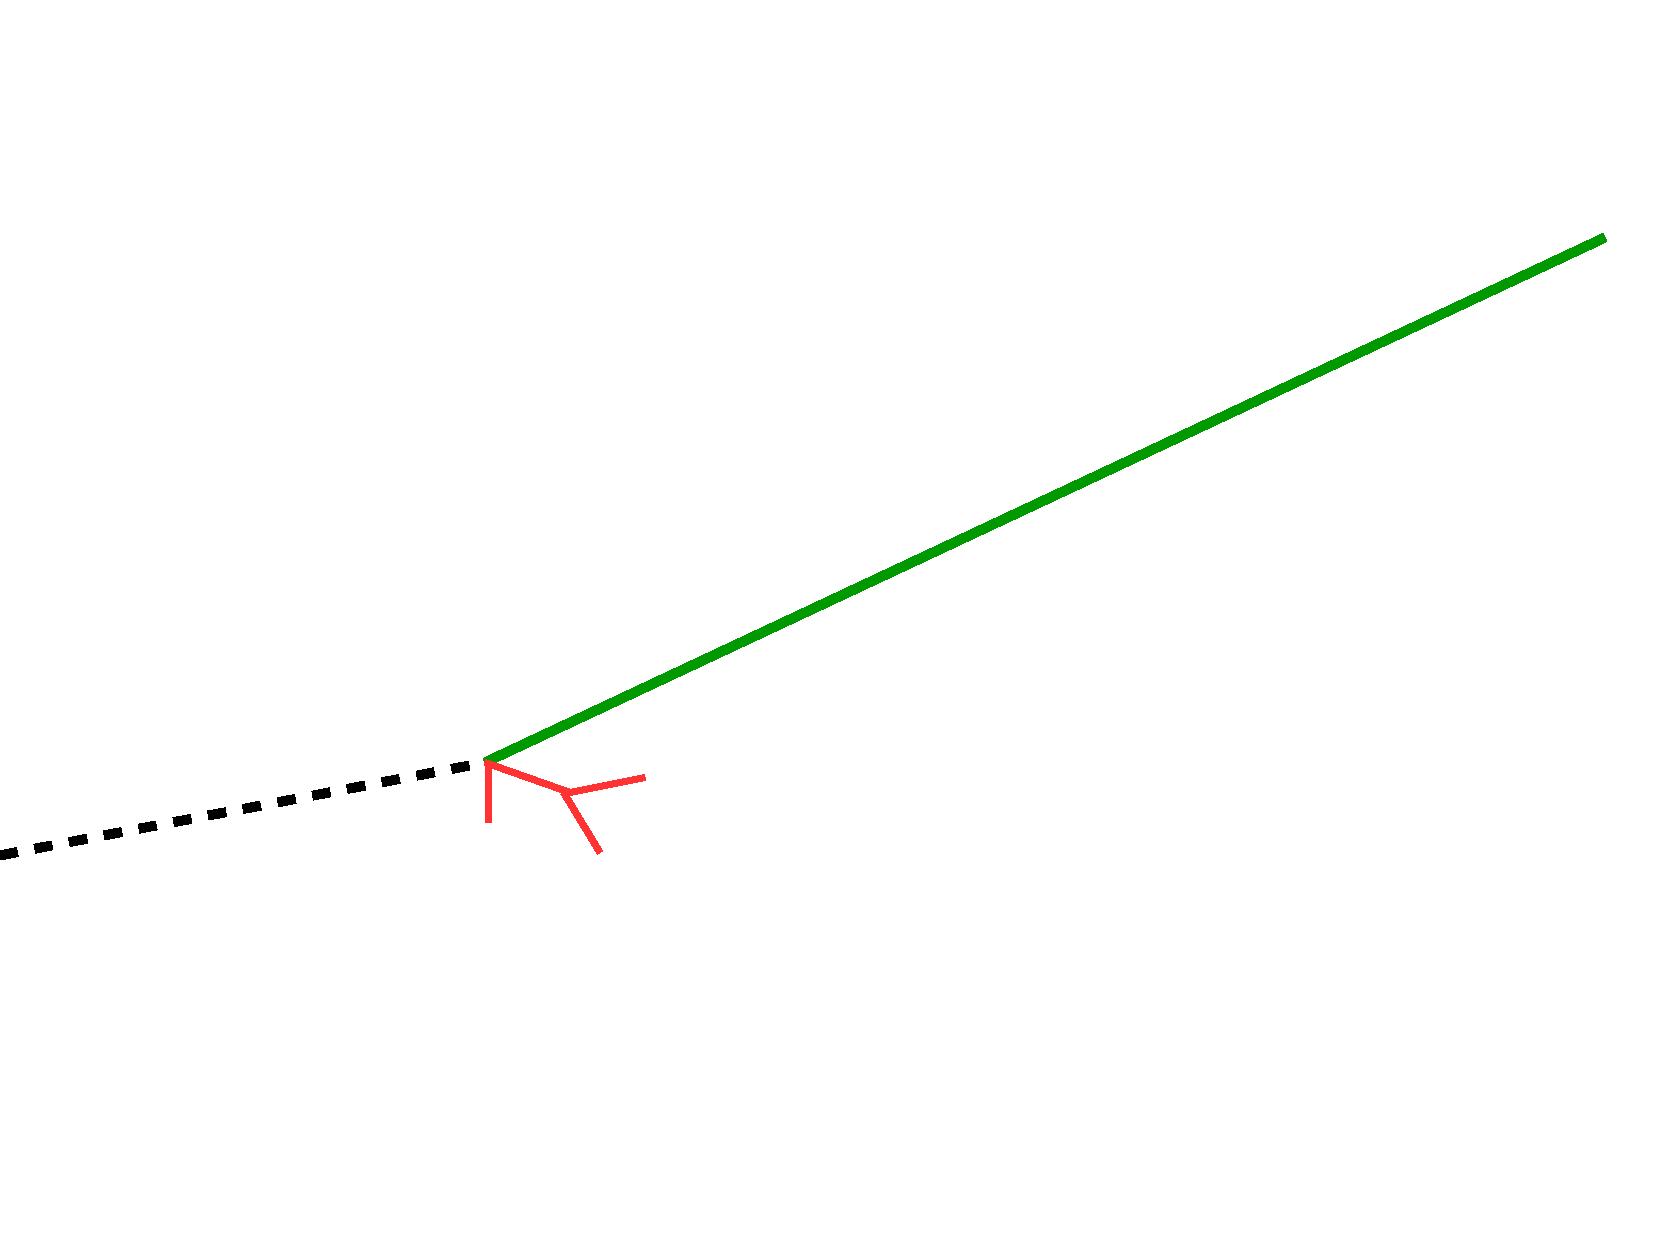
\includegraphics[width=2cm]{figures/neutrinos_properties/interaction_schematics/numu_CC_muon_only.pdf}
%             & $\mu^\pm$ track 
%             & Track-only  \\
%             \cmidrule{2-4} 
%             &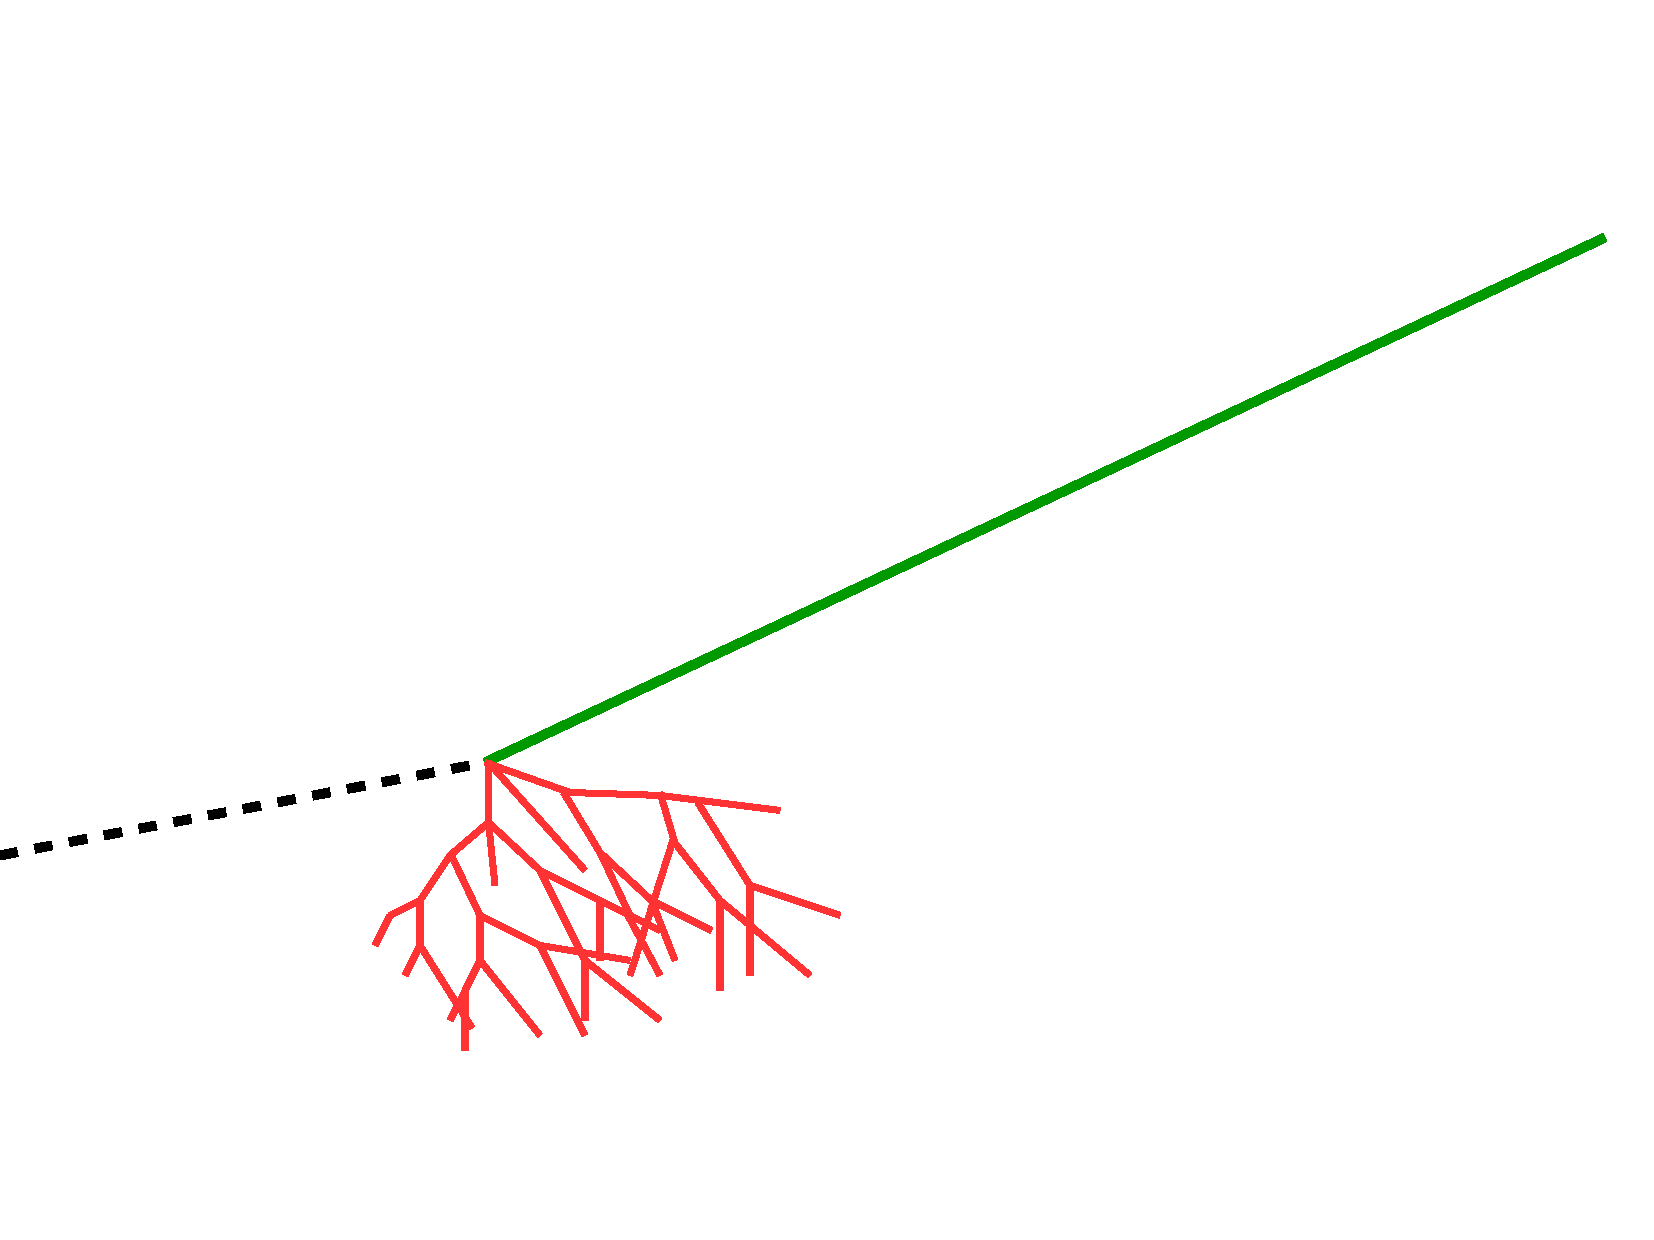
\includegraphics[width=2cm]{figures/neutrinos_properties/interaction_schematics/numu_CC_track_cascade.pdf}  
%             & $\mu^\pm$ track and hadrons 
%             & \multirow{2}{*}[-2em]{Track with cascade} \\
%             \cmidrule{1-3}
%             \multirow{2}{*}[-1.5em]{CC $\overset{\scriptscriptstyle(-)}{\nu_\tau}$ }
%             &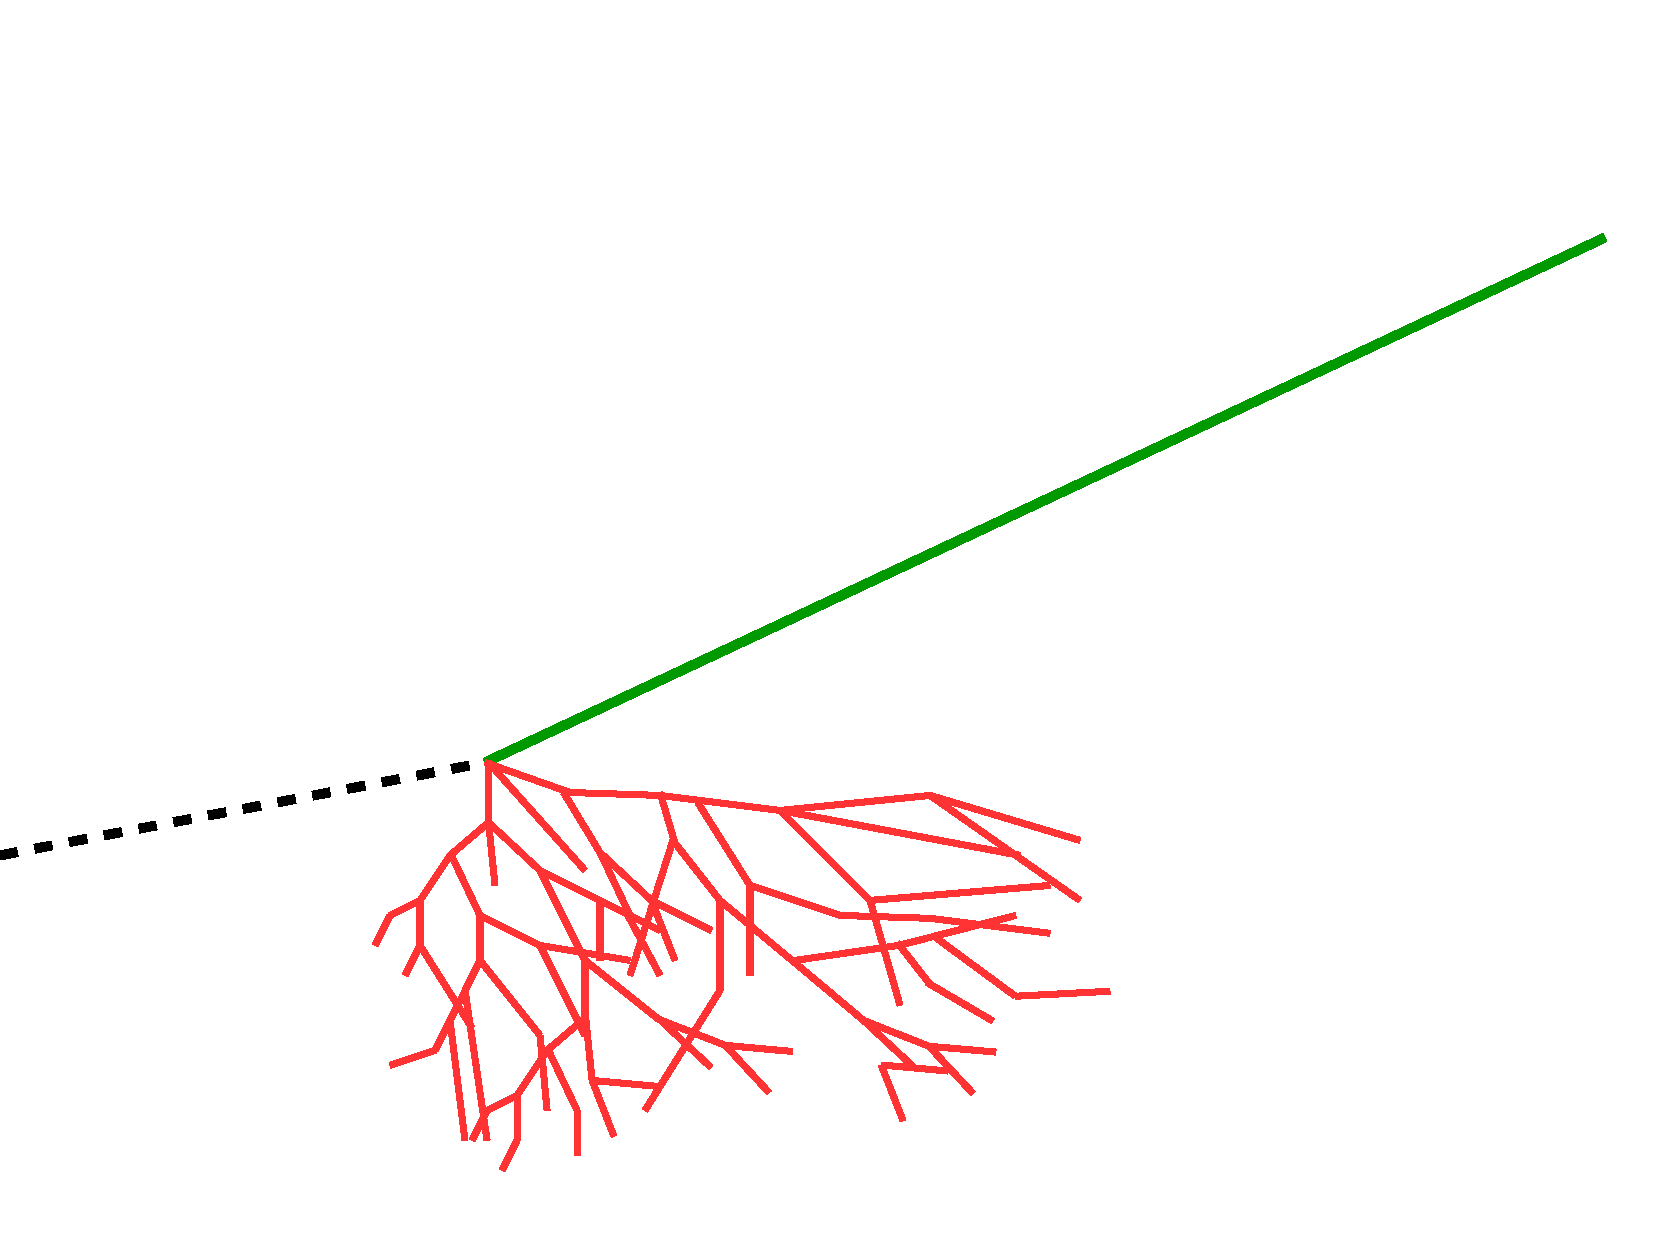
\includegraphics[width=2cm]{figures/neutrinos_properties/interaction_schematics/nutau_CC_track_cascade.pdf} 
%             & $\tau^\pm$ decaying into $\mu^\pm$ ($\sim$17\% BR), hadrons 
%             & {}\\
%             \cmidrule{2-4}
%             & 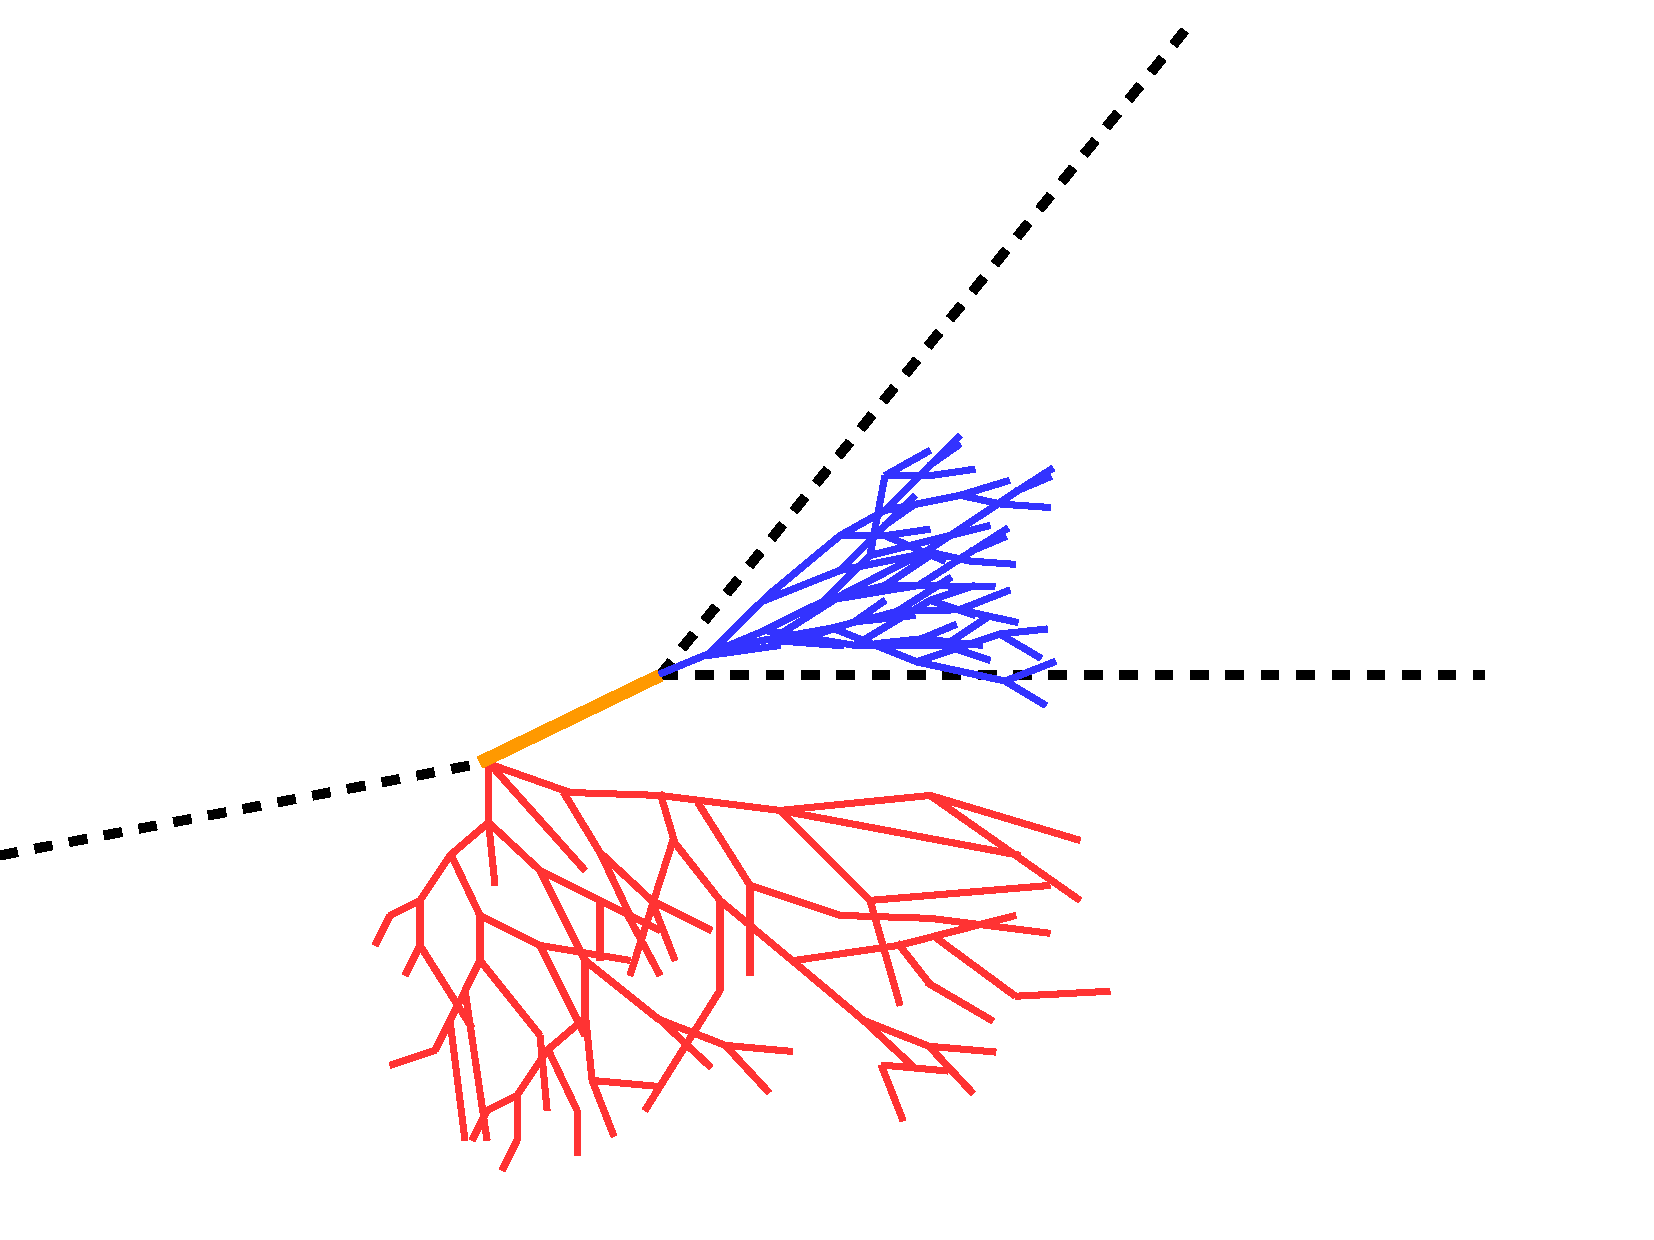
\includegraphics[width=2cm]{figures/neutrinos_properties/interaction_schematics/nutau_CC_cascadeonly.pdf}
%             & $\tau^\pm$ decaying into $e^\pm$ or hadrons ($\sim$83\% BR)  
%             & {}\\
%             \cmidrule{1-3} CC $\overset{\scriptscriptstyle(-)}{\nu_e}$ 
%             & 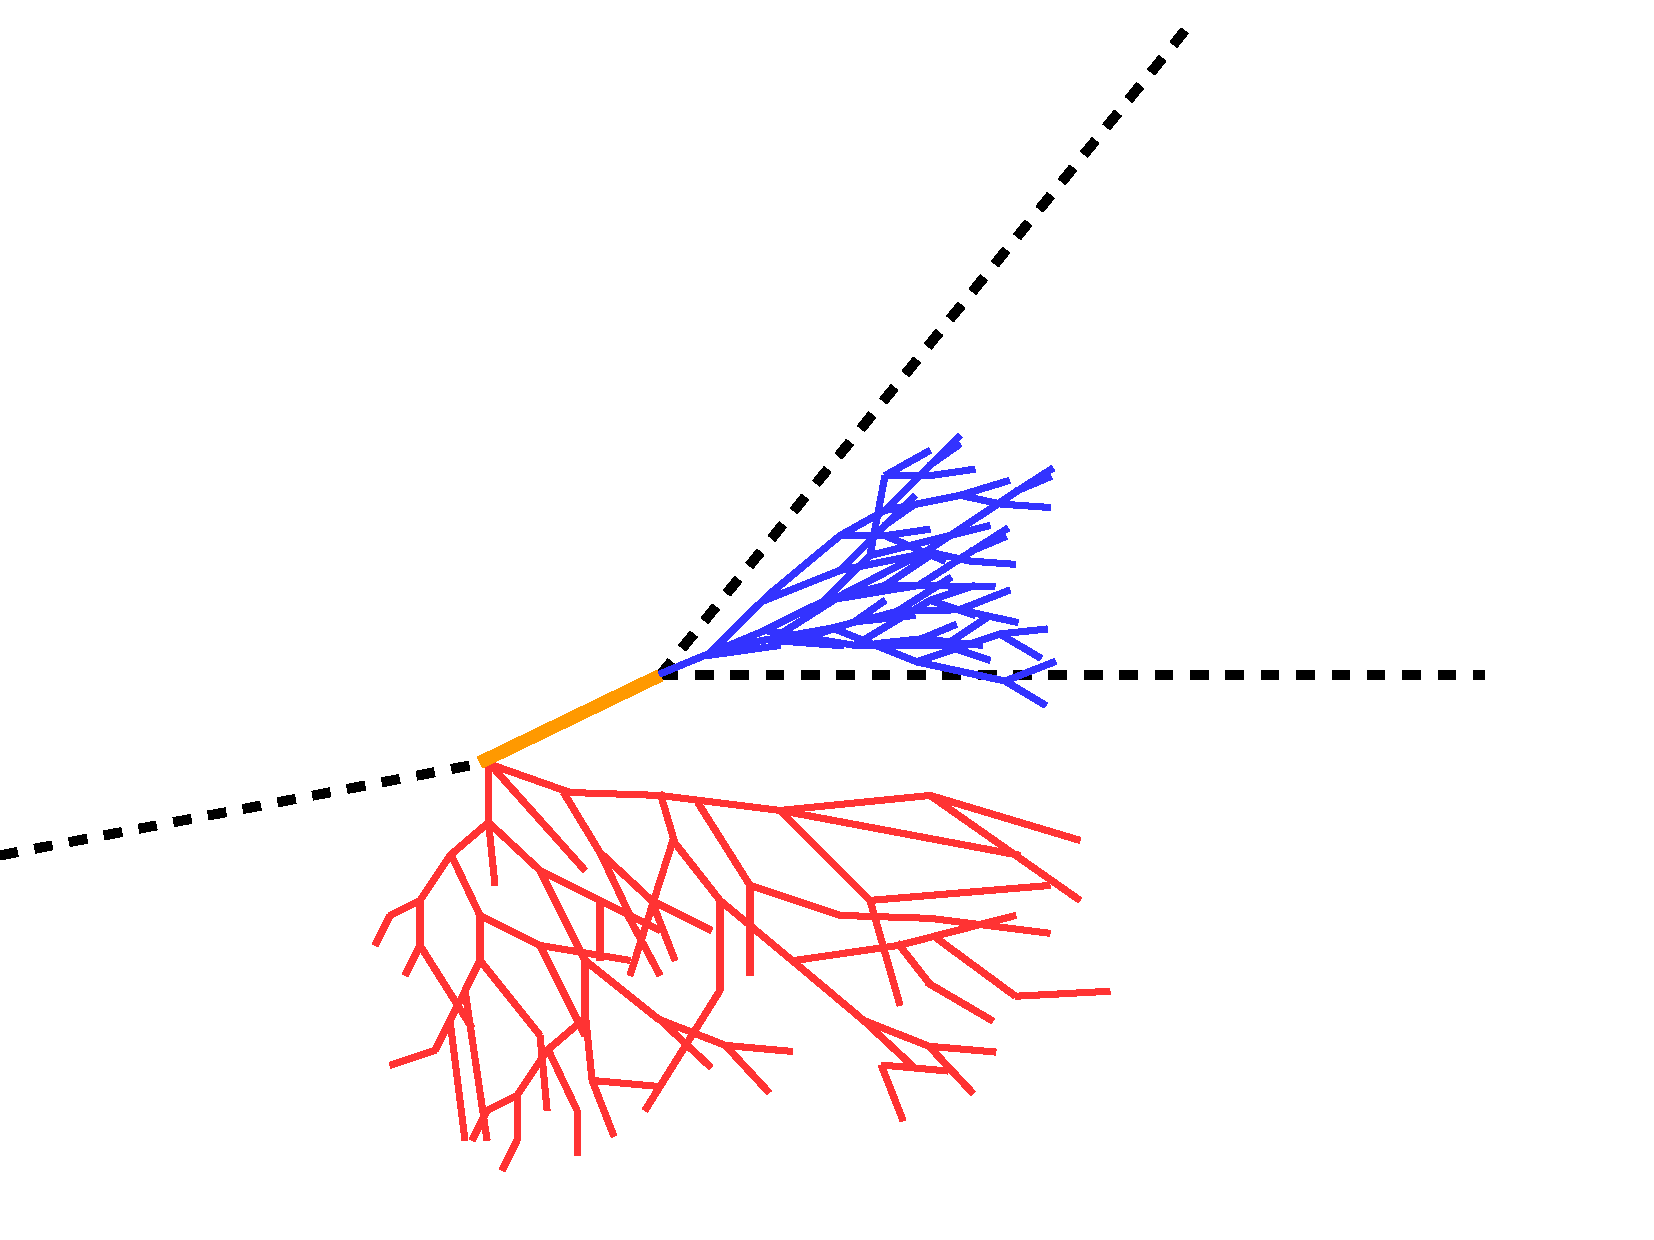
\includegraphics[width=2cm]{figures/neutrinos_properties/interaction_schematics/nue_CC_cascadeonly.pdf}
%             & $e^\pm$, hadrons & {Cascade-only}\\
%             \cmidrule{1-3}
%             NC $\overset{\scriptscriptstyle(-)}{\nu_\ell}$ 
%             & 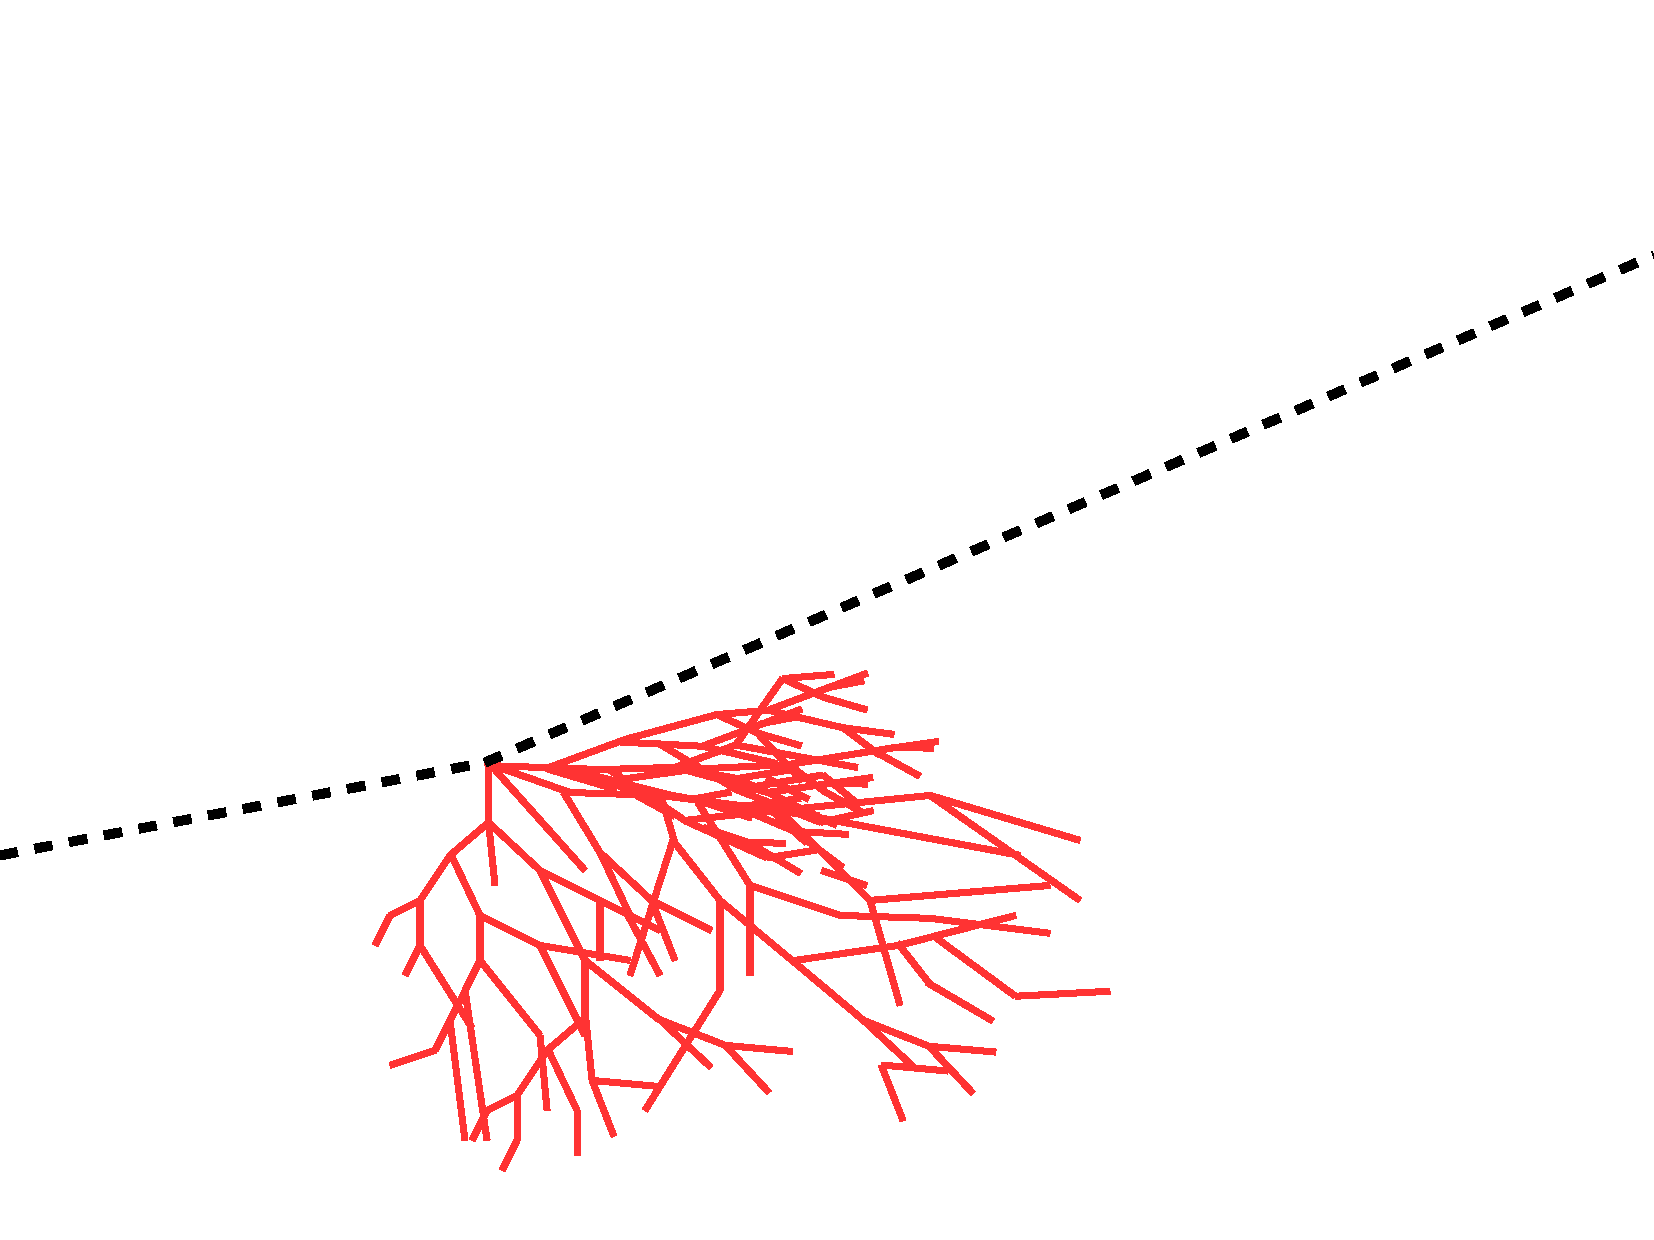
\includegraphics[width=2cm]{figures/neutrinos_properties/interaction_schematics/nuall_NC_cascadeonly.pdf} 
%             & hadrons &  {} \\
%             \hline
%         \end{tabular}
%     \end{center}
%     \caption[Event signatures in IceCube and their underlying interactions, taken from~\sidecite{ATerliuk}]{IceCube event signatures, their underlying interaction type and the particles that produce them. Also shown are the secondary particles produced in the interactions. Black dashed lines represent neutrinos, green lines muons, and blue and red lines are particles in electromagnetic and hadronic cascades, respectively. Taken from~\sidecite{ATerliuk}.}
%     \labtab{interactions_vs_signatures}
% \end{table}

The existence of the two types of event morphologies and their origins imply that by identifying track-like events we can identify events coming (mainly) from $\nu_\mu$-CC interactions and therefore obtain a flavor identification.
This is a crucial part of performing an oscillation analysis as will be further discussed in Section \refsec{analysis_principle}.

\subsubsection{Final Level Event Selection}

add this here or in the analysis chapters?


\section{Systematic Uncertainties} \labsec{systematic_uncertainties}

\subsubsection{Neutrino Cross-Section Systematic Uncertainties}


- three cross-section uncertainties are included, two for uncertainties in form factors of charged-current quasi-elastic (CCQE) and charged-current resonance (CCRES) events and for uncertainties in deep inelastic scattering (DIS) events

- the uncertainties in the form factors are due to uncertainties in the \textit{axial mass} $M_A$ which enters the form factor as in 

\begin{equation}
    F(Q^2) \sim \frac{1}{(1 - (\frac{Q}{M_A})^2)^2}
    \;,
\end{equation}
where $Q^2$ is the momentum transfer squared

\todo{which experiments measure the axial mass?}

- the axial mass can be determined experimentally and to include uncertainties on the values of $M_A^{CCQE}$ and $M_A^{CCRES}$, the cross-sections are computed with \textsc{GENIE} where the form factors are calculated varying the axial mass by $\pm 20\% (1\sigma)$/$\pm 40\% (1\sigma)$ around the nominal value
- this is an approximation of the recommended uncertainties by the GENIE collaboration, which are $-15\%$, $+25\%$ for $M_A^{CCQE}$ and $\pm 20\%$ for $M_A^{CCRES}$ \cite{genie}
- to apply a continuous uncertainty variation of the axial mass in a fit, the total cross-section is fit with a quadratic function to interpolate between the cross-sections computed with the different axial masses

\todo{add varied total cross-section for a few background HNL events}
\todo{add final level effects of varying the axial mass parameters (or example of one)}

- the uncertainty parameter of the DIS cross-section is based on the discrepancy between the cross-sections computed with GENIE and the ones computed with CSMS \sidecite{csms} above \SI{100}{giga\electronvolt}
- the included parameter scales the cross-section from the GENIE values to the CSMS values, which are considered more accurate above \SI{100}{giga\electronvolt}
- below \SI{100}{giga\electronvolt} the scaling is extrapolated linearly

\todo{add DIS systematic effect on final level histrograms}

\subsection{Atmospheric Flux}

\subsection{Detector Property Variations}

\subsubsection{Muon Uncertainties}

- final level muon fraction is below a percent
- just include a total scaling parameter in the analysis
(- total scale is degenerate with DOM efficiency, since increased DOM efficiency approximately leads to better muon rejection)
- changes in the muon spectral index have a negligible effect on the final level histograms and the analysis (see systematic impact test in section xx)

\todo{add muon systematic effects (total scale and ) on final level histrograms}
